\chapter{Methods}
Intro to chapter...
\label{chp:LIT}
\section{Calibration Methods Compared}
We compare the following calibration methods; Rejection Approximate Bayesian Computation (Rejection ABC), Sequential Approximate Bayesian Computation (Sequential ABC), … and Bayesian Maximum Likelihood estimation (BMLE). In the next sections, we will shortly explain each of these.

\subsection{Rejection ABC}
Rejection ABC is the most basic form of ABC. This method operates by sampling parameter values $(\theta_i,i = 1,… ,N)$ from the prior distribution $\pi(\theta)$  and given these sampled parameter values, data $(y)$ is simulated under a model. A summary statistic $(s)$ of the simulated data $(y)$ must satisfy a proximity criterion with the target statistic $(t)$ of the observed data $(x)$ such that $d(t,s ) \leq \epsilon$, where $d$ expresses the distance between the target and summary statistics $t$ and $s$, and $\epsilon$ represents a tolerance level. A target statistic is a data point from the observed data to be considered during the simulation procedure before a decision is made, as to whether a certain parameter combination is to be retained or discarded. The algorithm retains sampled parameter values for which the model produces simulated summaries $(s)$ that are closer to the target statistic $(t)$ than the tolerance $(\epsilon)$ \cite{sun}. Figure \ref{rej} illustrates how the rejection ABC algorithm functions. The simulator $(M)$ is run each time with a newly sampled parameter value $(\theta)$ from the prior distribution obtaining a simulated summary statistic. When the distance between a summary statistic and the target statistic $(y_\theta)$ is smaller than $(\epsilon)$; the parameter value is retained (red dot). Otherwise, it is discarded.

\begin{figure}[h!]
	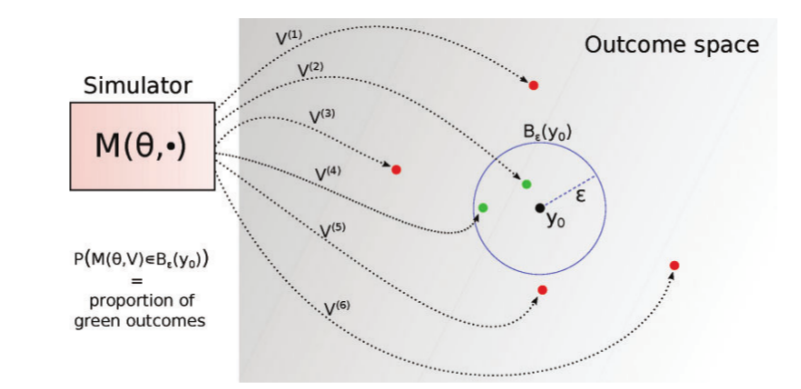
\includegraphics[width=\linewidth]{rej.png}
	\caption{Illustration of how the ABC Rejection algorithm works \cite{lint}.}
	\label{rej}
\end{figure}


From the Bayesian framework, estimation of the posterior distribution depends on the prior distribution and the likelihood. The posterior is defined as

\begin{equation}
\pi (\theta|x) = \frac{\pi (x|\theta) \pi (\theta))}{\pi (x)}
\label{e1}
\end{equation}


Since the denominator $\pi (\theta)$, which is the marginal probability of the data does not depend on $\theta$, the posterior can be expressed as proportional to the numerator, as shown in equation \ref{e2} below

\begin{equation}
\pi (\theta|x) = \pi (x|\theta) \pi (\theta)
\label{e2}
\end{equation}

Where $\theta$ is a vector of parameter values, $x$ is the observed data, $\pi (\theta|x)$ is the posterior distribution, $\pi (x|\theta)$ is the likelihood and $\pi (\theta)$ is the prior distribution. ABC techniques use this same knowledge in the approximation of the posterior. The distribution of the retained parameter values is expected to converge to the posterior distribution for arbitrarily small values of  the tolerance $(\epsilon)$ without the explicit calculation of the likelihood, such that

\begin{equation}
\pi (\theta|x) = \pi (\theta| d(t,s) \leq \epsilon)
\label{e3}
\end{equation}


\subsection{Sequential ABC}
Sequential ABC is a class of ABC methods that approximates the posterior progressively by drawing samples from the prior sequentially \cite{lenormand}. The prior for a particular sampling step depends on the previous retained sample except for the first sampling step which draws from the prior parameter space provided. Thus, the tolerance of the initial sampling step is less restrictive compared to the subsequent ones \cite{Mckinley}. The sample at the current sampling step $(S^{(t)} = \theta_{(i,i=1,…, N)}^{(t)})$ is derived from the previous sample $(S^{(t-1)})$ using a decreasing sequence of tolerance levels. These methods determine by themselves the tolerance level used at each sampling step and provide a stopping criterion \cite{lenormand}. This choice of tolerance for the current sampling step is determined as a function of the distances simulated in the previous sampling step \cite{Mckinley}. Figure \ref{seq} gives an illustration of how the sequential ABC algorithm works. The first step of sequential ABC is the same as running rejection ABC; simulator $(M)$ is run with parameter values $(\theta^{(1)})$ sampled from the prior distribution with tolerance  $(\epsilon_1)$ obtaining a simulated sample $(S^{(1)})$ and retained parameter values $(\theta_{r }^{(1)})$. In the second step, tolerance $(\epsilon_2)$ is decreased compared to tolerance $(\epsilon_1)$ and the prior is determined by the retained parameter combinations $(\theta_{r }^{(1)})$ in the first step. A second sample 〖$(S^{(2)})$ of parameter values is obtained at tolerance $(\epsilon_2)$  and this process is repeated until a stopping criterion is reached. At each sampling step, a decision is made whether to retain a particular parameter value or discard it. If a simulated summary statistic at that step is further from the target statistic $(y_0)$ than the tolerance level $(\epsilon_i)$ of that step, that particular parameter value is discarded, otherwise it is retained. The final sample $(S^{(N)})$〖aproximates the posterior distribution. 

\begin{figure}[h!]
	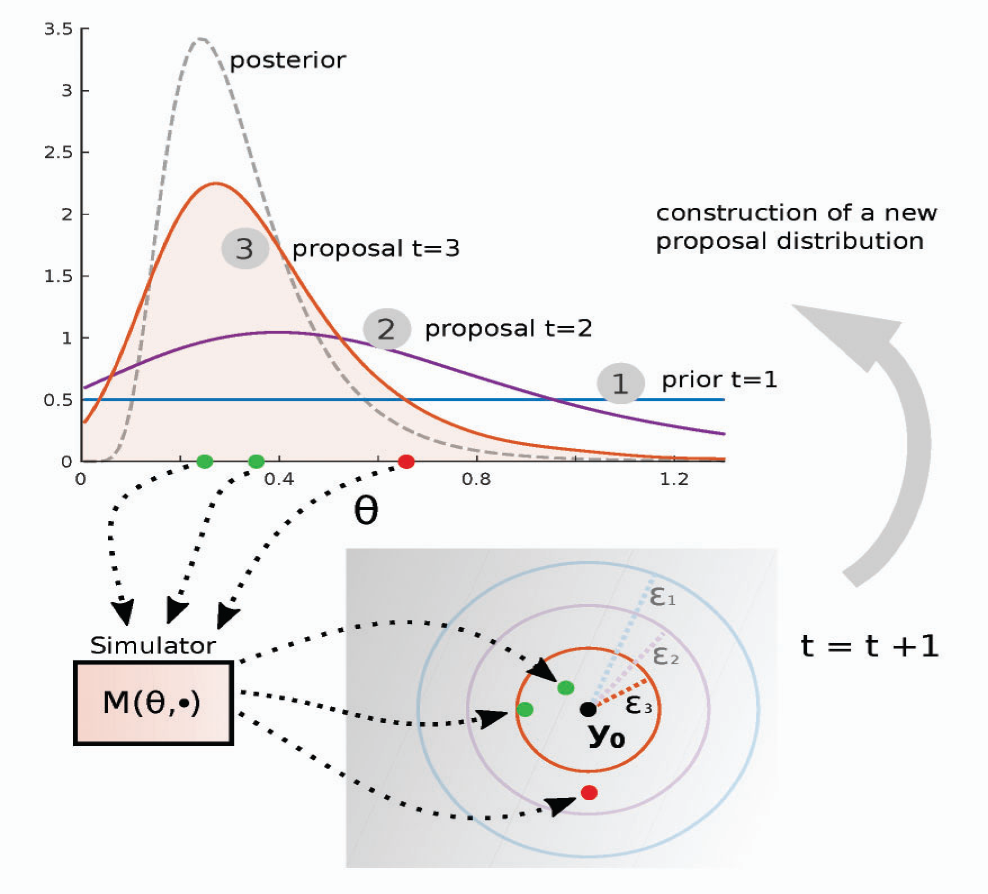
\includegraphics[width=\linewidth]{seq.png}
	\caption{Illustration of how the ABC Sequential algorithm works \cite{lint}.}
	\label{seq}
\end{figure}


\subsection{Bayesian Maximum Likelihood Estimation (BMLE)}

Bayesian Maximum Likelihood Estimation (BMLE) termed as “sampling from the posterior distribution” in \cite{Menzies}, approximates the posterior by applying sampling importance resampling. 
The Steps below describe the algorithm of BMLE and how the method is implemented.
\begin{itemize}
	\item 	Draw a large number of parameter combinations from the prior distribution
	\item For each parameter combination, run the model and estimate model outcomes
	\item Using these model outcomes, estimate the likelihood for the parameter combination and retain this value (log-likelihood)
	\item Resample from the original parameter sample with replacement, using the likelihood values as sampling weights.
\end{itemize}

The goodness-of-fit measure used in this model calibration method is the likelihood. Parameter combinations with high values of the likelihood are more consistent with the target supplied. This property allows the assessment of how the data supports one parameter combination compared with another. 

\section{The Simulation Model}
\subsection{The SIR Model}
The simulation model used in this study was a simple stochastic SIR (Susceptible - Infectious - Recovered) model, which we used to generate the observed data and applied to the methods. The SIR model is an epidemiological and compartmental model that computes the number of infectious individuals with an infectious disease in a closed population over time. A closed population implies that the population size remains constant over time, that is, there are no births and deaths. The population is divided into three compartments (i.e. health states) – susceptible, Infectious and recovered. The rates in between the compartments determine how many individuals move from one compartment to another.

\begin{figure}[h!]
	
\includegraphics[width=\linewidth]{sir_model.png}
	\caption{Structure of the simple SIR model.}
	\label{sir_model}
\end{figure}


This model involves a system of three non-linear ordinary differential equations (ODEs) that relates the number of susceptible $S(t)$, number of infectious $I(t)$, and number of recovered $R(t)$ individuals \cite{weiss}. The following system of ODEs governs the dynamics of the SIR model

\begin{equation}
\frac{dS}{dt} = -\beta SI 
\end{equation}

\begin{equation}
\frac{dI}{dt} = \beta SI - \gamma I
\end{equation}

\begin{equation}
\frac{dR}{dt} = \gamma I
\end{equation}


Where $\beta >0$ is the disease transmission rate, $\gamma >0$ is the recovery rate, $D_{inf} = \frac{1}{\gamma}$   is the duration of infection and $R_0 = \beta D_{inf}$ the basic reproductive number. $S$ is the proportion of individuals in the population that are susceptible to the disease and $I$ represents the proportion of infectious individuals. Susceptible individuals become infectious at a rate $\beta$. At a rate $\gamma$ , infectious individuals recover from the disease (gain permanent immunity to the disease) (LStone). 
The population stays constant throughout the transmission dynamics over the set time such that 
\begin{equation}
	S(t) + I(t) + R(t) = N
\end{equation}


Figure \ref{sir_model} illustrates the dynamics of a stochastic SIR model run in the R software over time $(t)$ of $75$ days for a population $(N)$ of $1000$ individuals. The blue curve indicates the Susceptible compartment, the red curve indicates the Infectious compartment and the green curve indicates the Recovered individuals. The susceptible compartment reduces to zero as the infectious compartment gradually picks up. 


\section{Performance Measures}
To compare the performance of the methods, we ran equal number of simulations for all methods per scenario and compared the resulting posterior to the reference posterior by computing percentage overlaps.

\subsection{Recording Efficiency (Computational Cost)}
To record how efficient each method is, we ran equal number of simulations for each model calibration method. For each scenario and calibration method, we recorded the total time taken to perform simulations and the time taken to run the SIR model in each calibration method. From these recorded times, we obtained the algorithm implementation times for each method as follows:

\begin{equation}
	\text{Algorithm implementation time} = \text{Total runtime} - \text{Model runtime}
\end{equation}

\subsection{Percentage Overlap}
To compare the posterior densities of the methods to the reference posterior density, we created a raster using the raster function from the raster library in R, which we used to compute percentage overlaps. A raster consists of a matrix of cells or pixels arranged into rows and columns to form a grid. Each cell contains a value which is the number of observations counted within a particular cell and represented by a color gradient. The raster was created by considering the minimum and maximum values of beta and gamma retained by the calibration methods to be compared as well as the reference. This was done so that the same raster could be applied to all the methods and reference. The resulting parameter space was divided into 100 x 100 equally sized bins with beta values on the x-axis and gamma values on the y-axis (see Figure \ref{raster}). This formed a grid in which the posterior densities laid. We applied the grid to each posterior density to quantify the density of each cell or pixel.

\begin{figure}[h!!]
	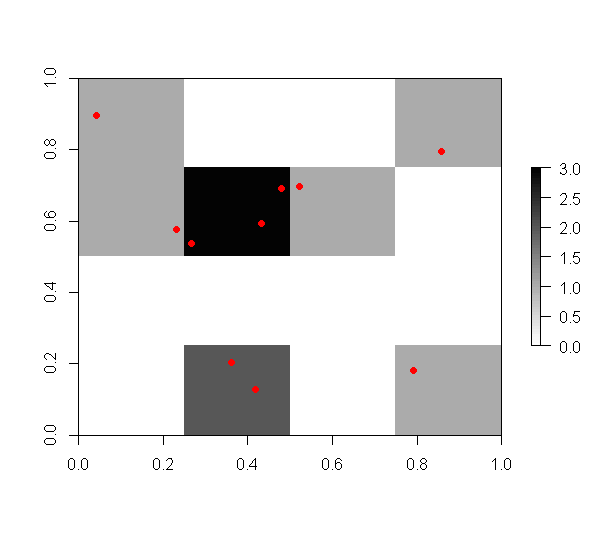
\includegraphics[width=\linewidth]{raster.png}
	\caption{4x4 raster applied to a posterior density.}
	\label{raster}
\end{figure}


The percentage overlap for each method was computed by summing the within cell density differences between the calibration method and the reference for that particular scenario and subtracting from 1. This was done such a way that, in the case of a perfect overlap between calibration method and the reference, percentage overlap goes to $1$ and in the case where there is no overlap between calibration method and the reference, percentage overlap goes to $0$ (see equation \ref{e4} below).

\begin{equation}
	P_{ij} = [1- \frac{(\sum|M_{ij} - R_i|)	}{2n}] x 100%
	\label{e4}
\end{equation} 


Where $P_{ij}$ is the percentage overlap for method $j$ and scenario $i$, $M_{ij}$ represents the matrix
form of the raster applied on calibration method $j$ and scenario $i$, $R_i$ represents the matrix
form of the raster applied on the reference for scenario $i$, $n$ is the number of parameter combinations retained by each calibration method.
